\section{File System}
Il file system é una parte del sistema operativo che si occupa di organizzare i file all'interno dei dischi

\subsection{I File}
Sono l'elemento principale per la maggior parte delle applicazioni, molto spesso, l'input di un' applicazione é un file;
quasi altrettanto spesso, l'output é un file, i file sopravvivono ai processi, il file system é una delle parti del sisema operativo che
sono piú importanti per l'utente, le propietá che il SO deve gesitre sono :
\begin{itemize}
    \item i file devono esistere a lungo termine
    \item condivisibilitá con altri processi (tramite nome simbolici)
    \item strutturabilitá (directory gerarchiche)
\end{itemize}
\subsubsection*{Gestione dei file}
I file sono gestiti da un insieme di programmi e librerie di utilitá, tali programmi sono gestiti in kernel mode, li
librerie vengono invocate come system call, ed hanno a che fare soprattuto con la memoria secondaria, inoltre
in linux é possibile gestire porzioni di RAM come se foessero file, Forniscono un'astrazionie sotto forma di operazionit tipiche
per ogni file vengono mantenuti degli attributi tipo nome permessi \ldots
\subsubsection*{Operazioni sui file}
\begin{itemize}
    \item Creazione (con annessa scelta del nome)
    \item Cancellazzione
    \item Apertura
    \item Lettura
    \item Scrittura
    \item Chiusura
\end{itemize}
le operazioni di dlettura é scrittura sono possibili solo se il file é stato aperto
\subsubsection*{Terminologia}
\begin{itemize}
    \item Campo (field)
    \item Record
    \item File
    \item Data Base
\end{itemize}
\subsubsection*{Campi}
\begin{itemize}
    \item dati di base
    \item contengono valori singoli
    \item caratterizzati da lunghezza e tipo di dato (o demarcazioni)
    \item esempio tipico: ASCII
\end{itemize}
\subsubsection*{Record}
\begin{itemize}
    \item Insieme di campi
    \item ognuno trattato come un'unitá
\end{itemize}
\subsubsection*{File}
\begin{itemize}
    \item Hanno un nome
    \item Sono insiemi di record correlati in ogni file ogni record é un solo campo con un byte
    \item Ogni file é trattato come unitá con nome propio
    \item possono implementare meccanismi di controllo di accesso
\end{itemize}
\subsubsection*{DataBase}
\begin{itemize}
    \item Sono un'opportuna collezione di file
    \item sono gestiti dai DBMS che sono processi di un sistema operativo
    \item Nei system operativi moderni non é piú necessario gestire File attraverso i data base
\end{itemize}
\subsubsection*{Sistemi per la gestione di file}
    \begin{figure}[H]
    \centering
    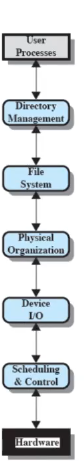
\includegraphics[width=0.2\textwidth]{immagini/FileSystemIO}
\end{figure}
I file managements Systems forniscono servizi agli utenti e alle applicazioni per l'uso di file e definiscono anche il modo in cui i
file sono usati, sollevando i programmatori dal dover scrivere codice per gestire i file
\subsection{Obbiettivi per il File Management Systems}
\begin{itemize}
    \item Rispondere alle necessita degli utenti riguardo alla gestione dei dati
    \item Garantire che i dati nei file siano validi
    \item Ottimizzare le prestazioni : sia dal punto di vista di throughput che tempo di risposta
    \item Fornire supporto per diversi tipi di memoria secondari
    \item minimizzare i dati per o distrutti
    \item Fornire un insieme di interfacce standard per i processi utente
    \item Fornire supporto per l'I/O effettuato da piú utenti in contemporaneamente
\end{itemize}
\subsubsection*{Requisiti}
\begin{enumerate}
    \item Ogni utente deve essere in grado di creare, cancellarem, leggere, scrivere e modificare un file
    \item Ogni utente deve poter accedere, in modo controllato, ai file di un altro utente
    \item Ogni utente deve poter leggere e modificare i permessi di accesso ai propri file
    \item Ogni utente deve poter ristrutturare i propri file in modo attinente al problema affrontato
    \item Ogni utente deve poter muovere dati da un file ad un altro
    \item Ogni utente deve poter mantenere una cop9ia di backup dei propri file (in caso di danno)
    \item Ogni utente deve poter accedere ai propri file tramite nomi simbolici
\end{enumerate}
\subsubsection{Directory}
Le directory contengono informazioni sui file (attributi,posizione,propietario) Una directory é essa stessa un file (speciale)
e fornisce il mapping tra i nomi dei file e i file stessi, un altro modo per chiamare gli attributi di un file é \textbf{metadati},
le operazione che sono possibili sulle directory sono:
\begin{itemize}
    \item Ricerca
    \item Creazione
    \item Cancellazione
    \item Lista del contenuto
    \item Modifica della directory
\end{itemize}
Le informazioni di base sono: il nome del file che deve essere unico per ogni directory,Tipo di file, Organizzazione del file, il
volume che indica il dispositvo su cui il file é memorizzato, indirizzo di partenza del file, dimensione attuale,dimensione allocata,
il propietario (puó dare i permessi di accesso), informazioni sull'accesso (potrebbe contenere username pasword per ogni utente autorizzato),
le Azioni permesse, poi ci sono anche i metadati sull'uso: Data di creazione, Identitá del creatore, Data dell'ultimo accesso in lettura
Data dell'ultimo accesso in scrittura, Identitá dell'ultimo lettore,Identitá dell'ultimo scrittore, Data dell'ultimo backup, Uso attuale (Lock,azione,correntte,\ldots)
\subsubsubsection{Struttura semplice per le Directory}
Inizialmente le directory era una lista di file, che rappresentava tutti i file presenti nel dispositivo
\subsubsubsection{Schema a due livelli}
Una directory per ogni utente, piú una (master ) che le contiene, la master contiene anche líndirizzo e le informazioni per
il controllo dell'accesso
\subsubsubsection{Schema ad albero}
Nello schema ad albero, é presente una directory master che contiene le directory utente, ed ogni directory utente contiene
a sua volta delle directory utente, questo schema é molto simile a quello a due livelli, ma permette una maggiore organizzazione.
\begin{figure}
    \centering
    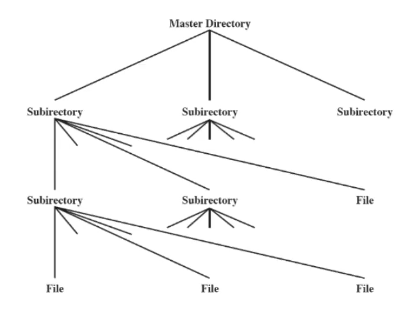
\includegraphics[width=0.2\textwidth]{immagini/DirectoryAlbero}
\end{figure}
\subsubsection{Nomi}
Gli utenti devono potersi riferire ad un file usando solo il suo nome, i nomi devono essere unici, ma un utente puó non avere
accesso a tutti i file, quello che succede siccome é presente una struttura ad albero c'é una directory di base (root) se
devo accedere ad una specifica directory devo specificare il percorso, che permette agli utenti di trovare i file, questo
permette di avere file con nomi uguali su directory diverse.
\begin{figure}[H]
    \centering
    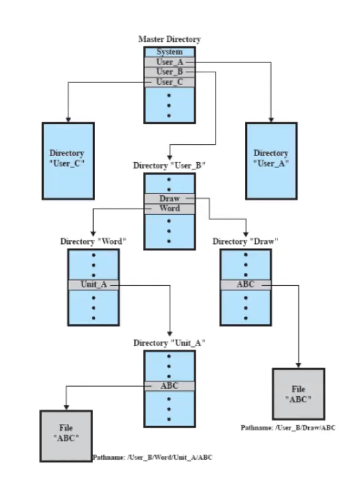
\includegraphics[width=0.6\textwidth]{immagini/EsempioAlberoNomiFile}
\end{figure}
\subsection{Directory di Lavoro}
A questo punto ogni volta che devo accedere ad un file dovrei specificare tutto il percorso dalla root directory fino al file,
per ovviare a questo problema é stata introdotta la directory di lavoro, quindi ogni processo ha una directory di lavoro
quindi chi ha bisogno di accedere ad un file, deve specificare solo il percorso relativo alla directory di lavoro.
\subsection{Gestione Della Memoria Secondaria}
Il SO é responsabile dell'assegnamento di blocchi a file, ci sono due problemi correlati:
\begin{itemize}
    \item decidere su quali byte del disco memorizzare i file
    \item mantenere traccia di dove ho memorizzato i file
\end{itemize}
Come si vede un problema é correllato all'altro, esistono tanti modi per farlo ogni modo definisce un nuovo file system,
i file si allocano in porzioni o blocchi, l'unitá minima é il settore del disco, ogni porzione o blocco é una sequenza contigua di
settori
\subsubsection{File Allocation}
ci sono diversi problemi d'affrontare:
\begin{itemize}
    \item pre-allocazione vs allocazione dinamica
    \item Porzioni di dimensione fissa o dinamice e quanto grandi
    \item Metodi di allocazione : contiguo, concatenato, indicizzato
    \item Gestione della file allocation Table
\end{itemize}
\subsubsection*{pre-allocazione vs allocazione dinamica}
La pre-allocazione vuol dire che: sto creando un file, sul disco alloco immediatamente la dimensione massima che il file
mi richiederá, nei file system che fanno uso di pre-allocazione, il file system deve sapere in anticipo la dimensione massima,
si intuisce che sistemi operativi moderni Linux\ldotsecc non fanno uso di pre-allocazione, in alcuni casi é stimabile
la dimensione massima di un file(Compilazione di un programma) in altri casi alcune applicazioni tendono a sovrastimare e quindi
si spreca spazio, per questo motivo l'allocazione dinamica é preferibile, quindi si comincia con una dimensione minima che é concessa
e mano a mano che aggiungo informazioni aggiusto la dimensione, per fare ció si usano due system call: \textbf{append} e \textbf{truncate}
\subsubsection*{Porzioni di dimensione fissa o dinamice e quanto grandi}
Abbiamo due possibilitá agli estremi:
\begin{itemize}
    \item Si alloca una porzione che é larga a sufficienza per l'intero file, questa soluzione é molto efficiente perché alloco in maniera contigua
    \item Si alloca un blocco alla volta, questa soluzione é molto efficiente per un sistema operativo che deve gestire molti file, ciascun blocco é una sequenza di n settori contigui
\end{itemize}
Per le prestazioni di accesso, é meglio per l'utente avere blocchi di grandi dimensioni, dal punto di vista del sistema operativo
potrebbe essere meno efficiente, fare porzioni molto piccole significa che la struttura dati che devo mantenere per tenere traccia
dei blocchi é molto grande, al contempo si facilitá la frammentazione.

Alla fine abbiamo 2 possibilitá:
\begin{itemize}
    \item Porzioni Grandi di dimensione  \textbf{variabile} : ogni singola allocazione é contigua, tabella di allocazione contenuta, complicata la gestione dello spazio libero: servono algoritmi ad hoc
    \item Porzioni fisse e piccole : tipicamente 1 blocco 1 porzione, molto meno contiguo del precedente, spazio libero (Guardare la tabella dei bit).
    \end{itemize}
Da notare che ci sono alcune combinazioni naturali, per esempio se sono in un sistema che fa pre- allocazioni, allora
faccio le porzioni grandi, essenzialmente per ogni file mi serve sapere solo dove inizia e dove finisce e quindi non ho bisogno
dellla tabella di allocazione, ogni file é quindi in un unica porzionie, e come per il porzionamento della RAM posso usare : best fit, first fit, next fit,
ma essendoci troppe variabili in questo caso non esiste un algoritmo migliore di un'altro, questo sistema é inefficiente per lo spazio
libero infatti necessita una periodica compattazzione e compattare il disco é molto piú oneroso che compattare la RAM perché é un I/O.
\subsubsection*{Metodi di allocazione}
\begin{figure}[H]
    \centering
    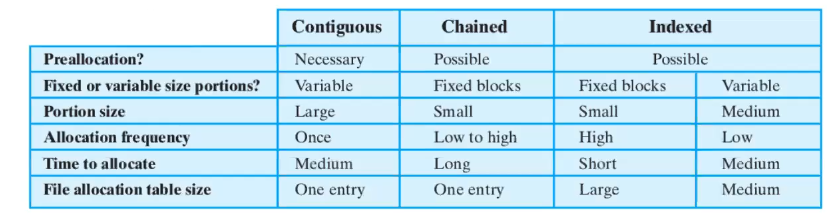
\includegraphics[width=0.6\textwidth]{immagini/MetodiDiAllocazione}
\end{figure}
Nella realtá si utilizzano questi tre metodi per allocare spazio:
\begin{itemize}
    \item Contiguo
    \item Concatenato
    \item Indicizzato
\end{itemize}
Ci sono per ciascuno di questi metodi ci sono delle caratteristiche, ad esempio se voglio fare allocazione
contigua la pre-allocazione é obbligatoria,Time to allocate indica l'overhead per il sistema operativo.
\subsubsection*{Contiguo}
Per allocare un file contiguo, significa che io conosco giá a priori la memoria che questo file richiederá, quindi
é necessaria la pre-allocazione, se un file prova a crescere oltre la dimensione massima, il sistema operativo
si rifiuta, é necessaria una sola entry nella tabella di allocazione dei file, inoltre sará presente frammentazione esterna.
\begin{figure}[H]
    \centering
    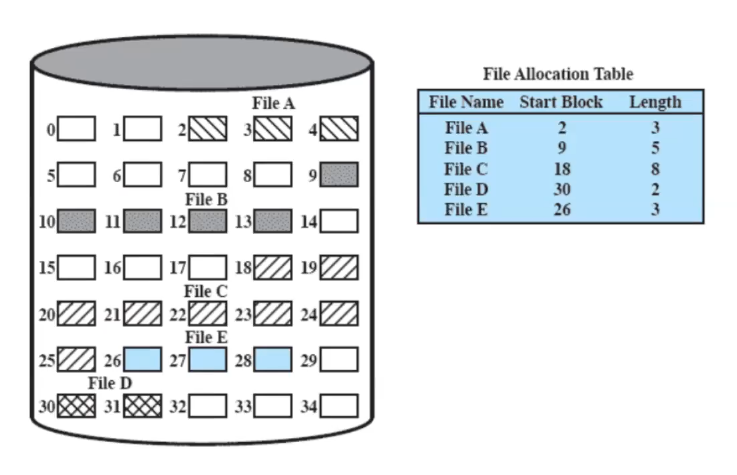
\includegraphics[width=0.5\textwidth]{immagini/AllocazioneContigua}
\end{figure}
Come si vede dall'immagine sopra i file sono tutti allegati in maniera contigua, e la FAT ha bisogno
di poche informazioni per tenere traccia di dove inizia e finisce il file, é presente lo stesso
problema presente nella ram ad esempio se arriva un file che richiede 8 settori contigui siamo costretti a
fare compattazzione, compattando si cambia la FAT.
\subsubsection*{Concatenata}
Abbiamo un allocazione di un blocco alla volta, il blocco é costiuito in 2 parti, una parte che contiene i file e una piccola
parte che contiente il puntatore al prossimo blocco, con questo modo non abbiamo piú frammentazione esterna quella interna
invece é trascurabile, questo modo va bene se dobbiamo accedere ad un file sequenzialmente, con il consolidamento serve per mettere
i blocchi il piú vicino possibile per migliorare le prestazioni.
\begin{figure}[H]
    \centering
    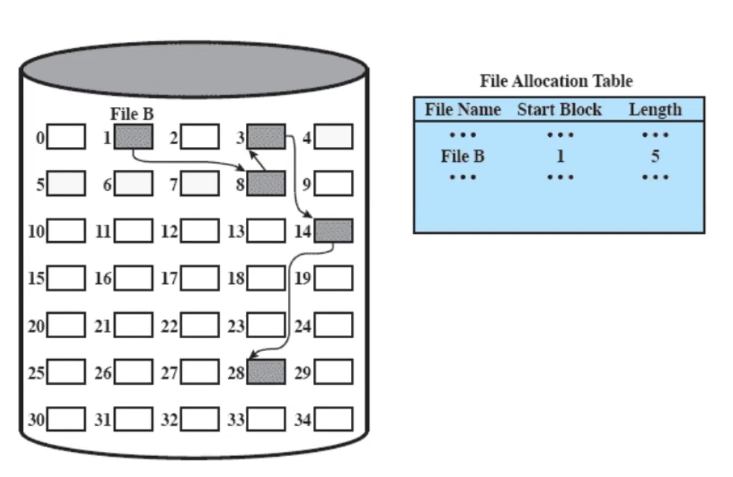
\includegraphics[width=0.5\textwidth]{immagini/AllocazioneConcatenata}
\end{figure}
\begin{figure}[H]
    \centering
    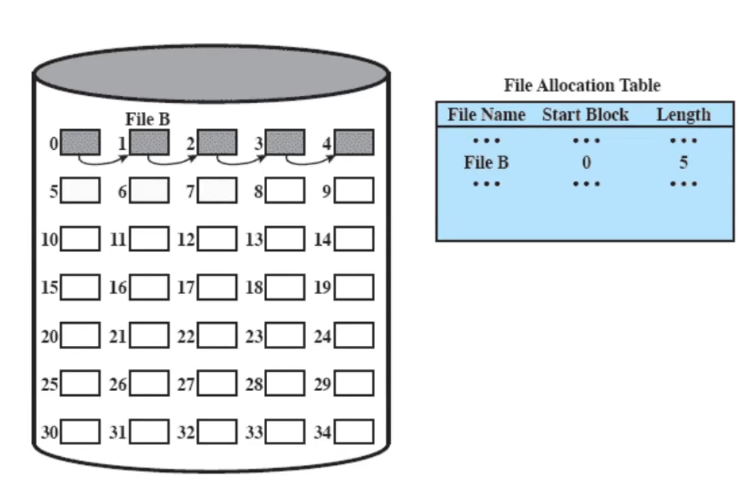
\includegraphics[width=0.5\textwidth]{immagini/AllocazioneDinamicaConsolidamento}
    \caption{Consolidamento}
\end{figure}
\subsubsection*{Indicizzata}
Quello che si utilizza nei file system moderni é l'allocazione indicizzata,
sostanzialmente fa una via di mezzo tra una allocazionie contigua e una concatenata, l'idea é
che ci sono dei blochi che contengono i dati ed altri che hanno dei puntatori.
\begin{figure}[H]
    \centering
    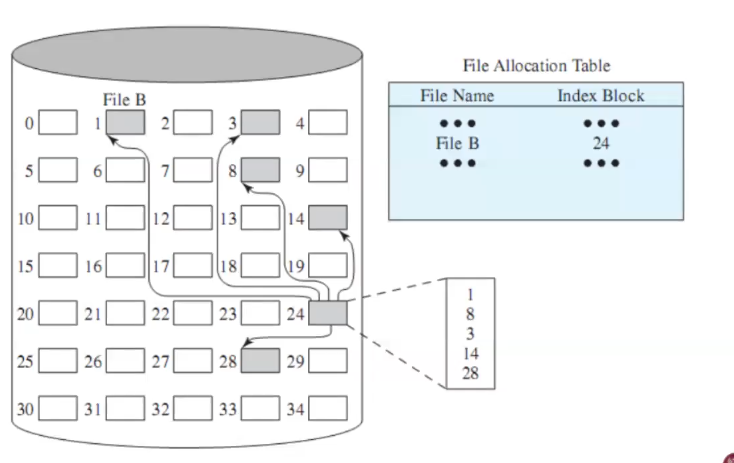
\includegraphics[width=0.5\textwidth]{immagini/AllocazioneIndicizzata}
\end{figure}
La File allocation table si limita a dire quale é il blocco indice di questo file, nel nostro caso il blocco 24 dove troviamo
tutti i puntatori ai blocchi che contengono i dati per quel determinato file.
\begin{figure}[H]
    \centering
    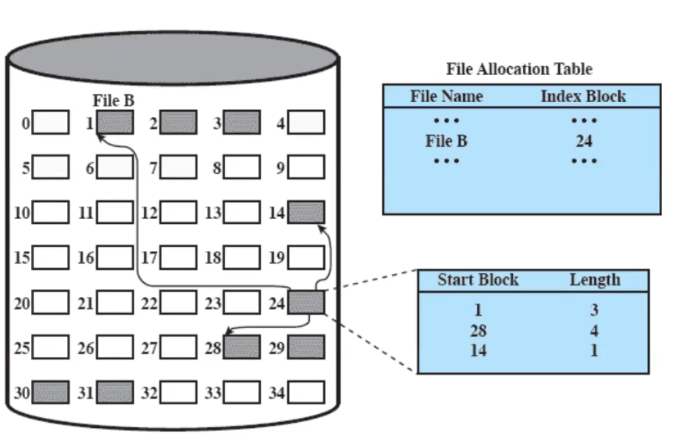
\includegraphics[width=0.5\textwidth]{immagini/AllocazioneIndicizzataVariabile}
    \caption{Allocazione indicizzata variabile}
\end{figure}
Nel caso in cui la lunghezza delle porzioni sia variabile il blocco indice deve contenere anche la lunghezza del
singolo tratto di blocchi contigui.

L'allocazione indicizzata puó essere fatta sia con blocchi di lunghezza fissa che con blocchi di lunghezza variabile,se si usa
la lunghezza fissa non abbiamo frammentazione esterna, ma se usiamo la lunghezza variabile abbiamo prestazioni migliori con rischi di
frammentazione esterna.
\subsection{Gestione dello Spazio Libero}
Per Gestire lo spazio libero, serve una tabella di allocazione di disco, oltre a quella di allocazione per i file ogni volta
che si alloca o cancella un file si deve aggiornare la tabella di allocazione, ci sono due metodi per tenere traccia dello spazio:
\begin{itemize}
    \item BitMap
    \item Lista di blocchi liberi
\end{itemize}
\subsubsection*{BitMap}
Faccio un vettore con un bit per ogni blocco su disco, va bene per tutti gli schemi visti finora, questo modo minimizza lo spazio richiesto,
ma il problema é che se il disco é molto pieno, la ricerca di uno spazio libero diventa molto lenta, si puó risolvere facendo delle tabella
riassuntive della tabella di bit, in modo da avere un'idea di dove cercare.
\subsubsection*{Porzioni libere concatenate}
Le porzioni libere concatenata sono una soluzione senza overhead di spazio, uso lo stesso sistema della allocazione concatenata solo per i
blocchi liberi, se c'é molta frammentazione esterna, le porzioni sono tutte da un blocco e la lista diventa molto lunga,occorre leggere un blocco libero per
saprere qual'é il prossimo, é dispendioso cancellare i file molto frammentati.
\subsubsection*{Lista dei blocchi liberi}
É presente una zona di memoria che va riservata, e ci metto una lista di indici (numeri di blocchi che sono liberi), potrebbe
sembrare poco intelligente, in realtá l'overhead puó essere molto basso, supponiamo che per ogni blocco bastano 4 bytes,
se mi servono 4 bytes per l'indirizzo ma i blocchi sono da 512 byte, richiede meno dell'1\% di spazio su disco, per avere parti della
lista in memoria principale si puó:
\begin{enumerate}
    \item organizzare la lista come pile, e tenere solo la parte alta
    \item pop per allocare spazio libero, push per deallocare spazio occupato
    \item quando la parte in memoria principale finisce, si prende una nuova parte da disco
    \item Funziona anche come coda
\end{enumerate}
\subsection{Volumi}
Un volume é un disco "logico" che sarebbe una partizione di un disco, oppure piú dischi assieme LVM, un insieme di settori in memoria secondaria,
che possono  essere usati dal SO o dalle applicazioni, i settori di un volume non necessariamente devono essere contigui.
\subsection{Dati e Metadati}
\subsubsection*{Consistenza}
I Dati sono il contenuto del file, mentre i metadati sono tutto il resto, i metadati devono essere tutti sul disco, per efficienza
dati e metadati possono essere in memoria principale quando si apre un file, c' é un problema di consistenza quando il file
é su RAM ovvero che risulta molto oneroso mantenere i metadati consistenti in tutte e due le memorie quindi l'aggiornamento
si fa solo quando il disco é poco usato e ci sono tanti aggiornamenti tutti insieme, ad oggi con il \textbf{Journaling} si é risolto
questo problema,anziché fare le modifiche on demand, quello che si fa é raccogliere in un file la lista di tutti i cambiamenti
che si devono fare e poi si fanno tutti insieme, in questo modo si evita di fare tanti accessi al disco, se c'é un crash
basta scrivere un bit all'inizio del disco, che dice se il sistema é stato correttamente spento o no, se non é stato spento
correttamente si esegue un porgramma per il ripristino del disco, con il journaling questo ripristino é piú facile pperché basta consultare il log.
\subsection{Gestione dei File in Unix}
In Unix ci sono 6 tipi di file:
\begin{itemize}
    \item normale
    \item directory
    \item speciale (mappano su nomi di file i dispositivi di I/O)
    \item named pipe (Per far comunicare due processi)
    \item hard link (Collegamenti, nome di file alternativo)
    \item symbolic link (Collegamenti simbolici)
\end{itemize}
\subsubsection*{Inode}
\begin{figure}[H]
    \centering
    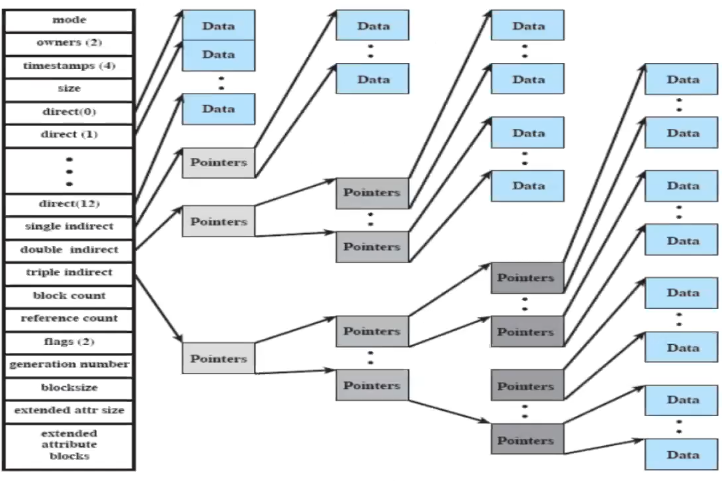
\includegraphics[width=0.6\textwidth]{immagini/Inode}
\end{figure}
In Unix si usa il concetto di Inode, che é un tipo particolare di allocazione indicizzata, i suoi dati sono organizzati in questo modo:
\begin{figure}[H]
    \centering
    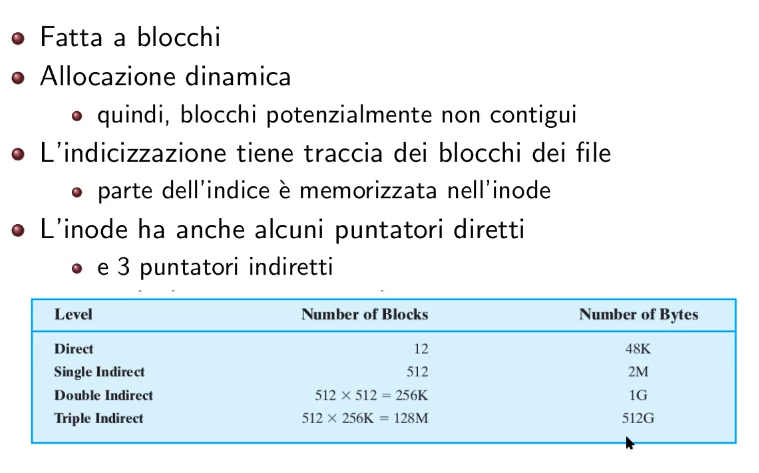
\includegraphics[width=0.6\textwidth]{immagini/Inode2}
\end{figure}